%% LyX 2.0.7.1 created this file.  For more info, see http://www.lyx.org/.
%% Do not edit unless you really know what you are doing.
\documentclass[letterpaper,english]{article}
\usepackage[T1]{fontenc}
\usepackage[latin9]{inputenc}
\usepackage{babel}
\usepackage{verbatim}
\usepackage{refstyle}
\usepackage{float}
\usepackage{fancybox}
\usepackage{calc}
\usepackage{bm}
\usepackage{amsthm}
\usepackage{amsmath}
\usepackage{fixltx2e}
\usepackage{graphicx}
\usepackage{esint}
\usepackage{xargs}[2008/03/08]
\usepackage[unicode=true,
 bookmarks=true,bookmarksnumbered=false,bookmarksopen=false,
 breaklinks=false,pdfborder={0 0 1},backref=false,colorlinks=false]
 {hyperref}
\hypersetup{pdftitle={Anytime Control: Model Predictive Control Approach},
 pdfauthor={Truong X. Nghiem}}

\makeatletter

%%%%%%%%%%%%%%%%%%%%%%%%%%%%%% LyX specific LaTeX commands.

\AtBeginDocument{\providecommand\figref[1]{\ref{fig:#1}}}
\AtBeginDocument{\providecommand\eqref[1]{\ref{eq:#1}}}
\AtBeginDocument{\providecommand\algoref[1]{\ref{algo:#1}}}
\AtBeginDocument{\providecommand\thmref[1]{\ref{thm:#1}}}
\AtBeginDocument{\providecommand\secref[1]{\ref{sec:#1}}}
\pdfpageheight\paperheight
\pdfpagewidth\paperwidth

\floatstyle{ruled}
\newfloat{algorithm}{tbp}{loa}
\providecommand{\algorithmname}{Algorithm}
\floatname{algorithm}{\protect\algorithmname}
\RS@ifundefined{subref}
  {\def\RSsubtxt{section~}\newref{sub}{name = \RSsubtxt}}
  {}
\RS@ifundefined{thmref}
  {\def\RSthmtxt{theorem~}\newref{thm}{name = \RSthmtxt}}
  {}
\RS@ifundefined{lemref}
  {\def\RSlemtxt{lemma~}\newref{lem}{name = \RSlemtxt}}
  {}


%%%%%%%%%%%%%%%%%%%%%%%%%%%%%% Textclass specific LaTeX commands.
  \theoremstyle{plain}
  \newtheorem{assumption}{\protect\assumptionname}
  \theoremstyle{definition}
  \newtheorem{problem}{\protect\problemname}
\theoremstyle{plain}
\newtheorem{thm}{\protect\theoremname}

%%%%%%%%%%%%%%%%%%%%%%%%%%%%%% User specified LaTeX commands.
\usepackage{fullpage}
\usepackage{algpseudocode}  % Of the algorithmicx package, flexible, more math-like
\usepackage{truonglatexdefs}
% Some useful math definitions, but not popular enough to be included in my official definition package.
% Copyright 2014 by Truong X. Nghiem (nghiem@seas.upenn.edu)

% \usepackage{xifthen}

%%%%%%%% Mathematical notations

\DeclareMathOperator{\diag}{diag}
\def\ones{\bm{1}}  % vector of 1's
\def\zeros{\bm{0}}  % vector of 0's
\def\IdentityMatrix{\mathbbm I}

\def\BallSet{\ensuremath{\BBBB}}  % Open ball

\DeclareMathOperator{\interior}{int}  % Interior

\DeclareMathOperator{\convhull}{co}  % Convex hull

\newcommand{\nullspace}[1]{\ensuremath{\ker\mleft(#1\mright)}}

\DeclareMathOperator{\dist}{dist}

\def\Given{\,|\,}

% This may conflict with the txfonts, pxfonts packages.
\def\coloneqq{\mathrel{\mathop:}=}
\def\definedas{\coloneqq}  % Alternatively, use \equiv for \definedas

\def\SuchThat{\,:\,}


%%%%%%%% Other definitions

\def\MATLAB{MATLAB\xspace}
\def\SIMULINK{SIMULINK\xspace}
\def\YALMIP{YALMIP\xspace}
\def\IPOPT{IPOPT\xspace}
\def\fmincon{\texttt{fmincon}\xspace}
\def\BMIBNB{BMIBNB\xspace}
\def\TrueTime{TrueTime\xspace}

%%%%%%%% Hyphenation rule
\hyphenation{MATLAB SIMULINK YALMIP IPOPT BMIBNB}


% Specific customizations for LyX
\newref{fig}{name=Figure~,Name=Figure~,names=Figures~,Names=Figures~}
\newref{eq}{name=Eq.~,Name=Eq.~,names=Eqs.~,Names=Eqs.~}
\newref{algo}{name=Algorithm~,Name=Algorithm~,names=Algorithms~,Names=Algorithms~}

\makeatother

  \providecommand{\assumptionname}{Assumption}
  \providecommand{\problemname}{Problem}
\providecommand{\theoremname}{Theorem}

\begin{document}
\newcommandx\sDelay[1][usedefault, addprefix=\global, 1=]{\delta_{#1}}
\newcommandx\sAccu[1][usedefault, addprefix=\global, 1=]{\epsilon_{#1}}


\global\long\def\XSet{\SSS}
\global\long\def\USet{\UUU}
\global\long\def\WSet{\WWW}
\global\long\def\WhSet{\widehat{\WSet}}
\global\long\def\ESet{\EEE}
\global\long\def\MPCProb#1{\PP_{#1}}


\global\long\def\ZSet{\ZZZ}


\global\long\def\Nom#1{\overbar{#1}}
\begin{comment}
Nominal variable
\end{comment}



\title{Anytime Control: the Model Predictive Control Approach}


\author{Truong~X.~Nghiem}


\date{\today}
\maketitle
\begin{abstract}
This technical report develops the theoretical results for a Model
Predictive Control approach for Anytime Control.
\end{abstract}

\section{System Model}

The control system consists of three components, interconnected as
illustrated in \figref{actual-system-diagram}:
\begin{enumerate}
\item The plant is a continous-time LTI system of the form
\begin{align}
\dot{x}(t) & =A_{c}x(t)+B_{c}u(t)+w_{c}(t)\label{eq:plant-cont-model}
\end{align}
where $x\in\RR^{n}$ is the state, $u\in\RR^{m}$ is the control,
and $w_{c}\in\RR^{n}$ is the process noise. The matrices $A_{c}$
and $B_{c}$ are system matrices of appropriate dimensions. Though
the process noise $w_{c}$ is unknown, we assume that it belongs to
a known compact and convex constraint set $\WSet_{c}\subset\RR^{n}$.
\item The estimator observes the output $y(t)=Cx(t)+v(t)$ of the plant
and estimates the current state of the plant, which cannot be measured
directly. Here $C$ is the output matrix and $v$ is the output noise.
Let $\hat{x}(t)$ denote the estimated state at time $t$ and $e(t)=x(t)-\hat{x}(t)$
the error between the actual and estimated states. Note that $e(t)$
is unknown, however it could usually be bounded, depending on the
characteristics of the estimation algorithm. The upper bound $\sAccu(t)$
of the norm $\norm{e(t)}$, where $\norm{\cdot}$ is any vector norm,
determines the \emph{accuracy} of the state estimation. The set of
error vectors corresponding to an accuracy $\sAccu\geq0$ is denoted
by $\ESet(\sAccu)\definedas\left\{ e\in\RR^{n}\SuchThat\norm{e}\leq\sAccu\right\} $.
We assume that there is a trade-off between the estimation accuracy
and its computation time, in particular the more accurate the estimation
is the longer it takes to compute, and conversely. The accuracy of
the estimator, hence its computation time, can be adjusted online
by changing its parameters or its algorithm.
\item The controller computes the control input for the plant as well as
adapts the estimator's accuracy to achieve a predefined control goal.
\end{enumerate}
\begin{figure}
\centering{}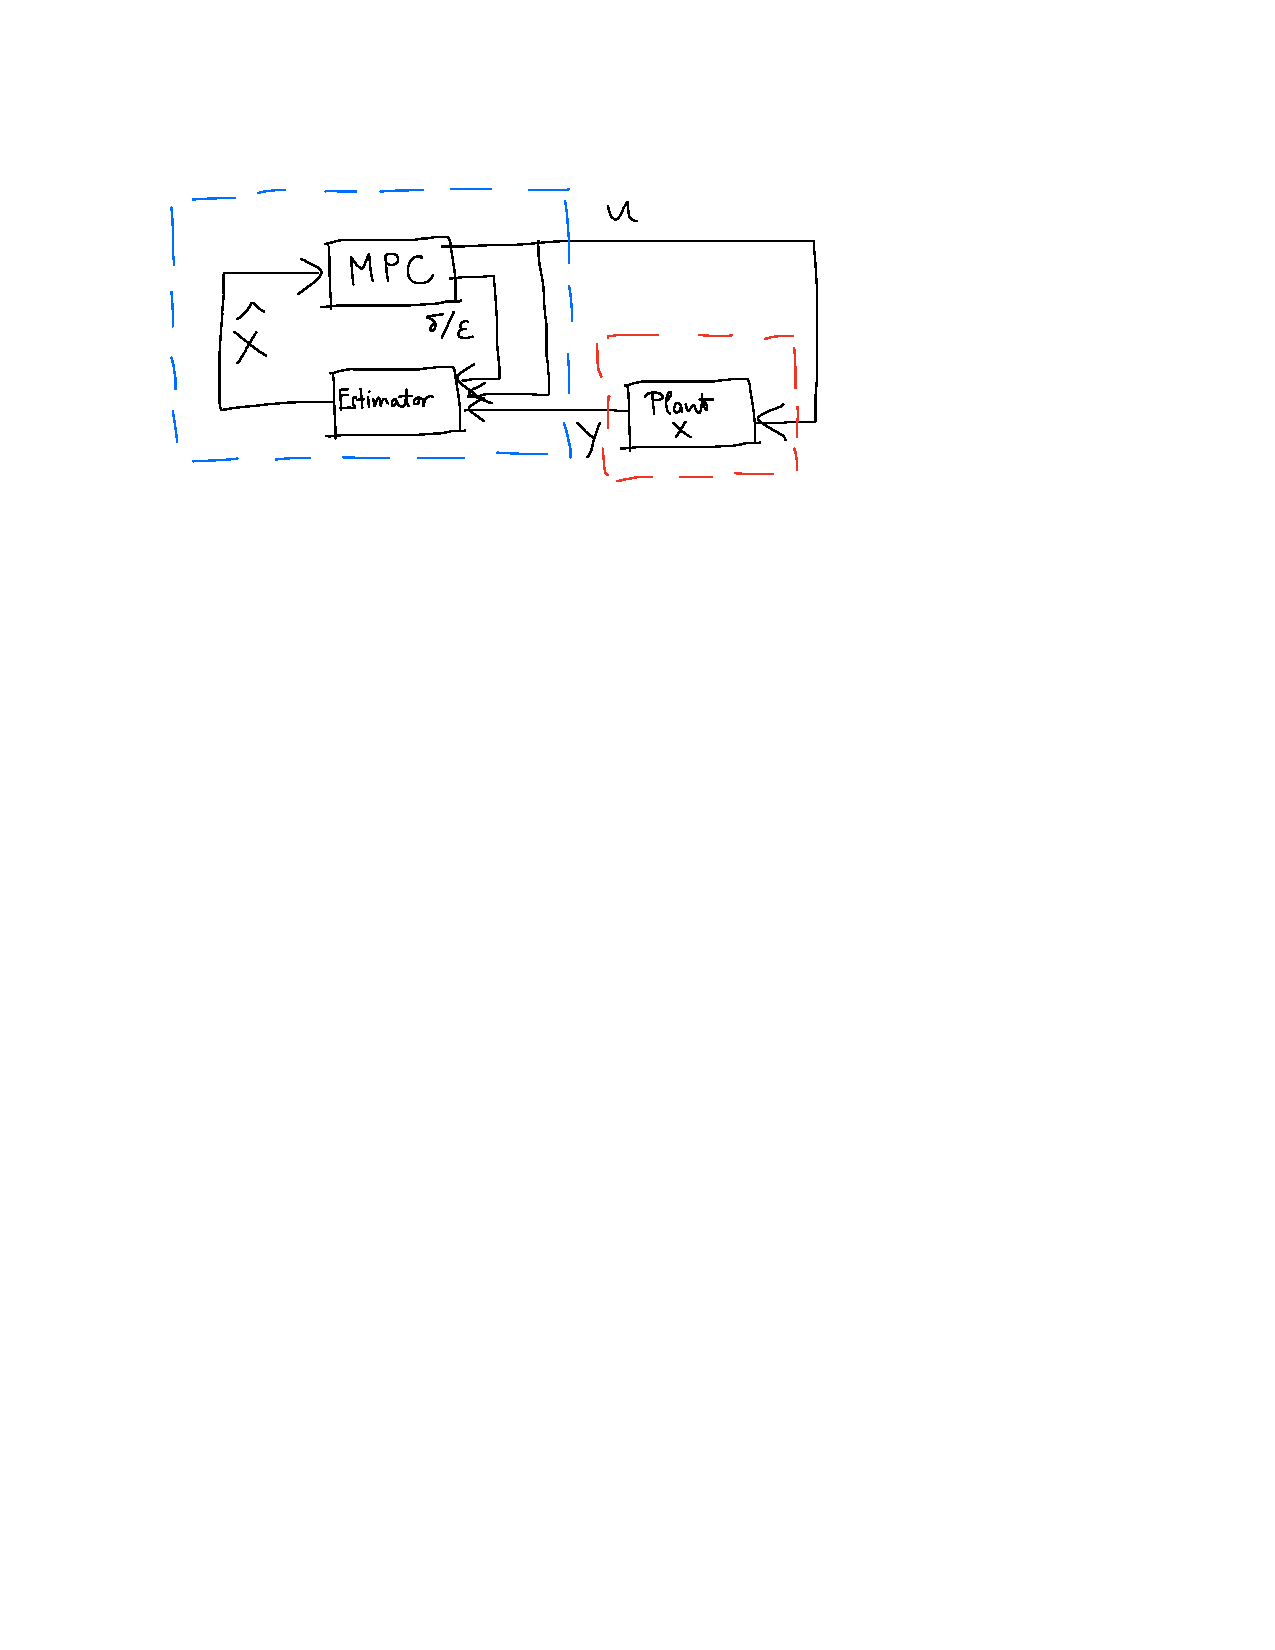
\includegraphics{figs/actual_system}\caption{Structural diagram of the control system.}
\label{fig:actual-system-diagram}
\end{figure}


The output $y(t)$ is sampled periodically at sampling instants $t_{s,k}=kT$,
where $k\in\ZZplus$ and $T>0$ is the predefined sampling period.
The sampled output is fed to the estimator which computes the state
estimate $\hat{x}_{k}\definedas\hat{x}(t_{s,k})$ with the desired
accuracy $\sAccu[k]\definedas\sAccu(t_{s,k})$ determined by the controller
in the previous time step. The controller then uses this state estimate
to compute the control input $u_{k}$ as well as decide on the desired
state estimate accuracy $\sAccu[k+1]$ for the next step. Let $\sDelay[k]$
be the worst-case total execution time of both the estimator and the
controller corresponding to the accuracy $\sAccu[k]$ of the state
estimation at time step $t_{s,k}$. We make the following theoretical
assumption of the state estimator.
\begin{assumption}
The estimation algorithm is given with a finite set of $p>0$ modes
(or options) $\Delta=\left\{ \left(\sDelay[i],\sAccu[i]\right)\right\} _{i=1}^{p}$;
each mode corresponds to a pair of time delay and estimation accuracy.
In each time step $k$, one of the estimation modes is selected, that
is $\left(\sDelay[k],\sAccu[k]\right)\in\Delta$.
\end{assumption}
This assumption means that in this paper we will not design nor analyze
the estimation algorithm; in other words, the estimator is a black-box
given to us with known characteristics. Furthermore, the control implementation
is subject to the following assumption.
\begin{assumption}
[Time-triggered actuation]The control actuation is delayed by $\sDelay[k]$,
\ie the control variable computed by the controller is applied exactly
at the actuation instant $t_{a,k}=t_{s,k}+\sDelay[k]$.
\end{assumption}
The order of sensing\textendash{}computing\textendash{}actuating and
their timing are illustrated in the diagram in \figref{timing-diagram}.
We note that in each step $k\geq0$, the estimation accuracy $\sAccu[k]$
and hence the delay $\sDelay[k]$ are already decided in the previous
step and known to the controller. The previous control input $u_{k-1}$
is still used until $t_{a,k}$ when the new control input $u_{k}$
is computed and applied by the controller. The controller also chooses
the next desired accuracy $\sAccu[k+1]$ and delay $\sDelay[k+1]$
to be used in the next step $k+1$. In the first step $k=0$, the
initial accuracy $\sAccu[0]$, the initial delay $\sDelay[0]$, and
the initial control input $u_{-1}$ are chosen by the designer.

\begin{figure}
\begin{centering}
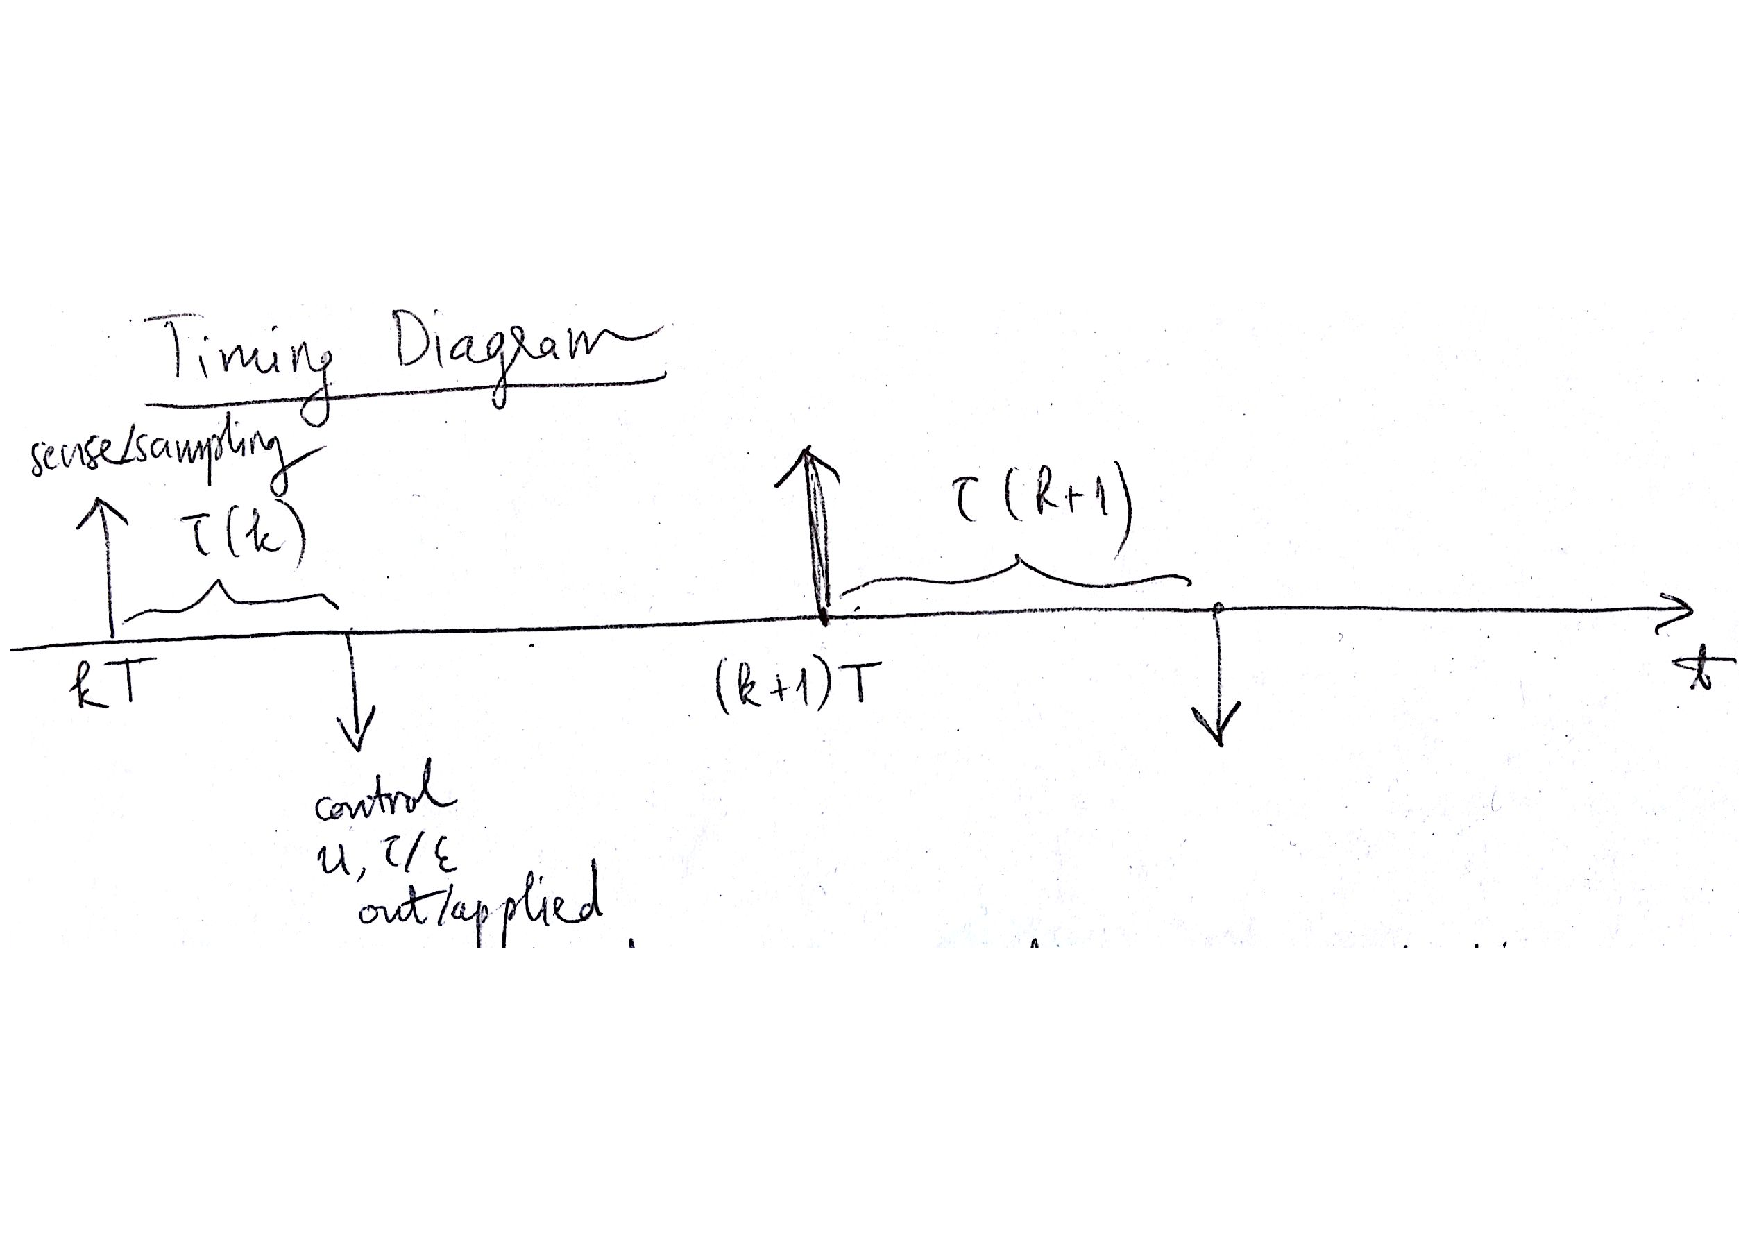
\includegraphics[width=0.8\columnwidth]{figs/timing}
\par\end{centering}

\caption{Timing diagram of Anytime Control.}
\label{fig:timing-diagram}
\end{figure}



\subsection{Discrete-time System Dynamics}

The plant's state at each sampling time $t_{s,k}$ can be described
by the discrete-time system:
\begin{equation}
x_{k+1}=Ax_{k}+B_{1}(\sDelay[k])u_{k-1}+B_{2}(\sDelay[k])u_{k}+w_{k},\qquad k\geq0\label{eq:disc-dynamics}
\end{equation}
in which
\begin{gather*}
A=\eu^{A_{c}T},\quad w_{k}=\int_{t_{s,k}}^{t_{s,k+1}}\eu^{A_{c}(t_{s,k+1}-t)}w_{c}(t)\diff t=\int_{0}^{T}\eu^{A_{c}(T-t)}w_{c}(t_{s,k}+t)\diff t\\
B_{1}(\sDelay[k])=\int_{t_{s,k}}^{t_{a,k}}\eu^{A_{c}(t_{s,k+1}-t)}B_{c}\diff t=\int_{0}^{\sDelay[k]}\eu^{A_{c}(T-t)}B_{c}\diff t\\
B_{2}(\sDelay[k])=\int_{t_{a,k}}^{t_{s,k+1}}\eu^{A_{c}(t_{s,k+1}-t)}B_{c}\diff t=\int_{\sDelay[k]}^{T}\eu^{A_{c}(T-t)}B_{c}\diff t\text{.}
\end{gather*}
Here $w_{k}$ is the accumulated process noise during the interval.
Because $w_{c}(t)$ is constrained in the compact set $\WSet_{c}$
and $T$ is finite, we can find a compact and convex set $\WSet$
that bounds $w_{k}$, that is
\begin{equation}
w_{k}\in\WSet\qquad\forall k\geq0\text{.}\label{eq:disturb-constraint}
\end{equation}
We remark that both the current control $u_{k}$ and the previous
control $u_{k-1}$ appear in the dynamics in \eqref{disc-dynamics}.
Furthermore, the input matrices $B_{1}(\sDelay[k])$ and $B_{2}(\sDelay[k])$
depend on the delay $\sDelay[k]$; hence $\sDelay[k]$ is also an
input to the dynamics. The estimation accuracy $\sAccu[k]$ does not
appear in the equation because it only affects the state estimate
$\hat{x}_{k}$ which is used by the controller to compute $u_{k}$;
therefore $\sAccu[k]$ indirectly affects the dynamics via the control
input.


\subsection{State and Control Constraints}

For every step $k\geq0$, the actual state of the plant $x_{k}\definedas x(t_{s,k})$
must satisfy a safety condition that 
\begin{equation}
x_{k}\in\XSet\label{eq:state-constraint}
\end{equation}
where $\XSet\subset\RR^{n}$ is the set of safe states. We assume
that $\XSet$ is a polytope of the form $\XSet\definedas\left\{ x\in\RR^{n}\SuchThat Hx\leq b\right\} $,
where matrix $H$ and vector $b$ constitute an H\textendash{}representation
of $\XSet$%
\begin{comment}
citation
\end{comment}
. Note that $\XSet$ is not necessarily bounded. In addition, a control
input $u_{k}$ is only valid if it belongs to the predefined set of
admissible controls $\USet\subseteq\RR^{m}$, that is
\begin{equation}
u_{k}\in\USet\qquad\forall k\geq0\text{.}\label{eq:input-constraint}
\end{equation}
The sets $\XSet$ and $\USet$ are part of the problem statement and
are either chosen by the designer or determined by physical constraints
of the plant and the actuators.


\subsection{Control Performance}

The goal of the controller is two fold: it needs to maintain the state
and control constraints while minimizing a cost function given by
\[
J=\sum_{k=0}^{\infty}\left(\ell(x_{k},u_{k})+\pi(\sDelay[k])\right)
\]
where $\ell(\cdot)$ is the stage cost function for the state and
control, and $\pi(\cdot)$ is the stage cost function for the estimation
and computation. Typically a longer execution time $\sDelay[k]$ will
result in a higher computation cost $\pi(\sDelay[k])$. For example,
if the state estimation involves capturing an image by a camera then
detecting and locating an object from the image, a longer computation
time might correspond to a higher resolution of the image, more data
to be transmitted and processed, and more power consumed for communication
and computation. These stage cost functions are chosen by the designer
to achieve a desired control performance.


\subsection{Control Problem}

The control problem is stated as follows.
\begin{problem}
\label{prob:control-problem}Design a feedback controller, which computes
the admissible control input $u_{k}\in\USet$ and the required estimation
accuracy $\sAccu[k+1]$ (equivalently the delay $\sDelay[k+1]$) based
on the current state estimate $\hat{x}_{k}$, to minimize the cost
$J$ while maintaining the state constraint $x_{k}\in\XSet$ for all
$k\geq0$.
\end{problem}

\subsection{Notations}

In the rest of this paper, we use the following notational convention.
We write $x_{j\Given k}$ for a variable $x$ at time step $j$ in
the RMPC optimization for time step $k\leq j$ (\ie the prediction
made at time step $k$ of variable $x$ at time step $j$). To emphasize
that this variable depends on an independent variable $v$ we write
$x_{j\Given k}(v)$; however in many cases, for brevity, we will only
write $x_{j\Given k}$ when the dependency is implicitly understood.
The set of possible disturbance $\hat{w}_{k}=w_{k}+Ae_{k}-e_{k+1}$
depends on the estimation accuracy at steps $k$ and $k+1$ and is
denoted by $\WhSet(\sAccu[k],\sAccu[k+1])$, \ie $\WhSet(\sAccu,\sAccu')\definedas\left\{ w_{k}+Ae_{k}-e_{k+1}\SuchThat w_{k}\in\WSet,e_{k}\in\ESet(\sAccu),e_{k+1}\in\ESet(\sAccu')\right\} $.
Note that we assume $\WhSet(\sAccu[k],\sAccu[k+1])$ is independent
of the time step $k$. %
\begin{comment}
The computation of this set will be discussed later in the implementation.
\end{comment}
{} It can be computed as $\WhSet(\sAccu,\sAccu')=\WSet\oplus A\ESet(\sAccu)\oplus\left(-\ESet(\sAccu')\right)$
where the symbol $\oplus$ denotes the Minkowski sum of two sets.
We use $\IdentityMatrix_{n}$ to denote the identity matrix of size
$n\times n$. The notation $\bm{0}_{n}$ ($\bm{1}_{n}$) represents
the column vector of length $n$ whose elements are all 0's (respectively
1's). Similarly, $\bm{0}_{n\times m}$ ($\bm{1}_{n\times m}$) is
the matrix of size $n\times m$ whose elements are all 0's (1's).
Sometimes, when the dimensions of the vectors or matrices are clear
from the context, we omit the subscripts for brevity.


\section{Anytime Control Robust MPC}

In this paper, we design the controller using a Robust Model Predictive
Control (RMPC) approach via constraint restriction \cite{chiscietal01swp,richardsetal05rmp}.
In order to ensure robust safety and feasibility, the key idea of
this approach is to tighten the state constraint iteratively to account
for possible effect of the disturbances. As time proresses, this ``robustness
margin'' is used in the MPC optimization with the nominal predictions,
\ie the original dynamics where the disturbances are either removed
or replaced by nominal disturbances. An advantage of this approach
is that, because only the nominal dynamics are used, the complexity
of the optimization is the same as for the nominal problem.

Since the controller only has access to the state estimate $\hat{x}_{k}$
but not the plant's state $x_{k}$, conceptually the control system
structure is arranged as in \figref{conceptual-system-diagram}. From
the controller's point of view, the\emph{ plant }that it controls
consists of both the physical plant, whose state is hidden, and the
estimator, whose state is exposed to the controller. This composed
plant is called a \emph{virtual plant}. Although the exact state $x_{k}$
is hidden from the controller, it is within an unknown but bounded
distance from the state estimate. With this knowledge, the controller
can compute the control input so that robust safety and feasibility
are achieved, and it can also adjust the estimation accuracy appropriately.

\begin{figure}
\centering{}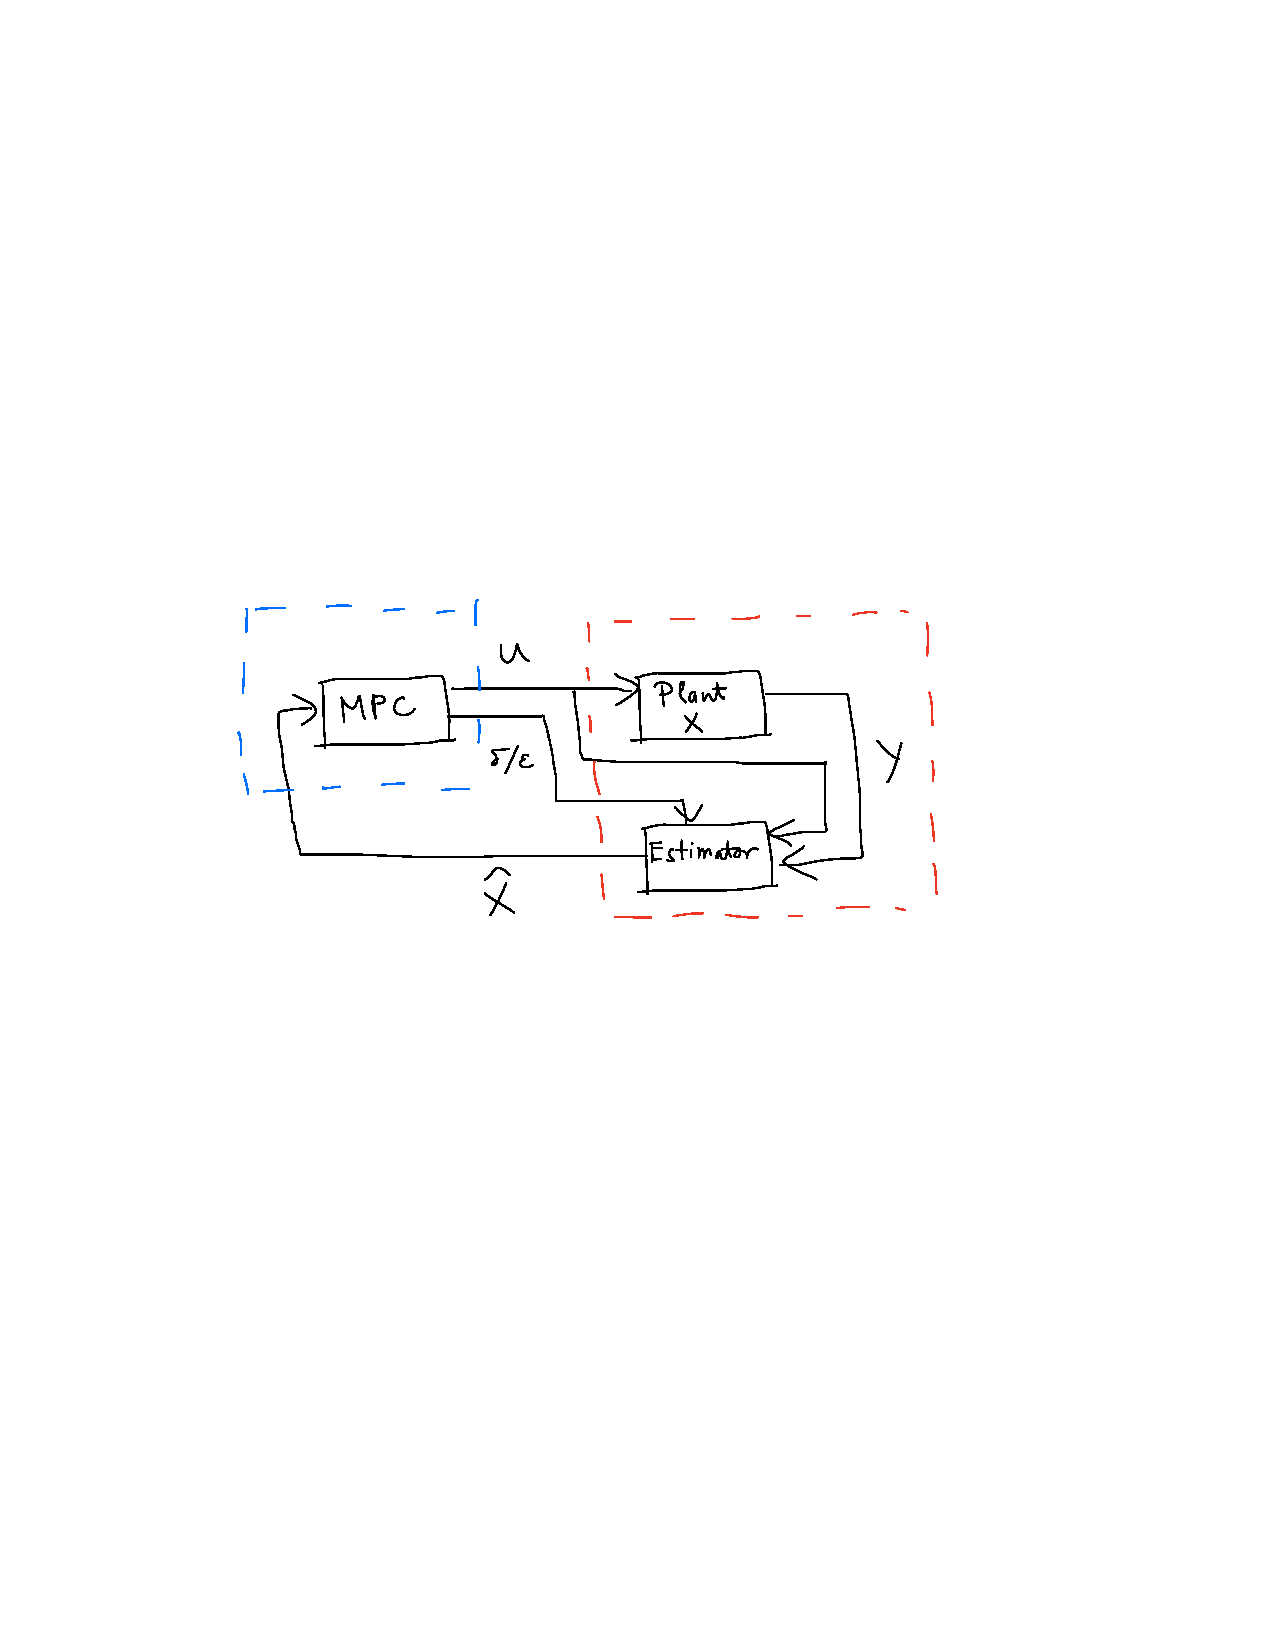
\includegraphics{figs/conceptual_system}\caption{Conceptual structural diagram of the control system for control design.}
\label{fig:conceptual-system-diagram}
\end{figure}


Because the exposed state of the virtual plant is $\hat{x}$ we need
to rewrite the plant's dynamics with respect to $\hat{x}$. The error
between $ $$x_{k}$ and $\hat{x}_{k}$ is $e_{k}=x_{k}-\hat{x}_{k}$.
At time step $k+1$ we have
\begin{align*}
\hat{x}_{k+1} & =x_{k+1}-e_{k+1}\\
 & =Ax_{k}+B_{1}(\sDelay[k])u_{k-1}+B_{2}(\sDelay[k])u_{k}+w_{k}-e_{k+1}\text{,}
\end{align*}
 then, by writing $x_{k}=\hat{x}_{k}+e_{k}$, we obtain the dynamics
\begin{equation}
\hat{x}_{k+1}=A\hat{x}_{k}+B_{1}(\sDelay[k])u_{k-1}+B_{2}(\sDelay[k])u_{k}+\hat{w}_{k},\quad k\geq0\label{eq:estimator-dynamics}
\end{equation}
 where $\hat{w}_{k}=w_{k}+Ae_{k}-e_{k+1}$.

\shadowbox{\begin{minipage}[t]{1\columnwidth}%
Truong: It's important to note here that I used $e_{k}=x_{k}-\hat{x}_{k}$,
so the implementation code should be double checked to match this
definition.%
\end{minipage}}

The dynamics in \eqref{estimator-dynamics} has an nonstandard form
where it depends on both the current and the previous control inputs.
However we can expand the state variable to store the previous control
input as
\[
\hat{z}_{k}=\begin{bmatrix}\hat{x}_{k}\\
u_{k-1}
\end{bmatrix}\in\RR^{n+m}
\]
and rewrite the dynamics as, for all $k\geq0$,
\begin{equation}
\hat{z}_{k+1}=\hat{A}(\sDelay[k])\hat{z}_{k}+\hat{B}(\sDelay[k])u_{k}+\hat{F}\hat{w}_{k}\text{.}\label{eq:estimator-std-dynamics}
\end{equation}
Here, the system matrices%
\begin{comment}
, which depend on the delay $\sDelay[k]$,
\end{comment}
{} are
\begin{equation}
\hat{A}(\sDelay[k])=\begin{bmatrix}A & B_{1}(\sDelay[k])\\
\bm{0}_{m\times n} & \bm{0}_{m\times m}
\end{bmatrix},\quad\hat{B}(\sDelay[k])=\begin{bmatrix}B_{2}(\sDelay[k])\\
\IdentityMatrix_{m}
\end{bmatrix},\quad\hat{F}=\begin{bmatrix}\IdentityMatrix_{n}\\
\bm{0}_{m\times n}
\end{bmatrix}\text{.}\label{eq:lifted-matrices}
\end{equation}


Let the actual expanded state is $z_{k}=\left[x_{k}^{T},u_{k-1}^{T}\right]^{T}$.
Because the expanded state consists of both the plant's state and
the previous control input, the state constraint $x_{k}\in\XSet$
and the control constraint $u_{k}\in\USet$ are equivalent to the
joint constraint $z_{k}\in\XSet\times\USet$. We can now describe
the RMPC algorithm for the dynamics in \eqref{estimator-std-dynamics}.


\subsection{Tractable RMPC Algorithm}

Let $N\geq1$ %
\begin{comment}
May need to change the smallest N
\end{comment}
{} be the horizon length of the RMPC optimization. Because the system
matrices in the state equation~(\ref{eq:estimator-std-dynamics})
depend nonlinearly on the variables $\sDelay[k]$, the RMPC optimization
is generally a mixed-integer nonlinear program, which is very hard
to solve. To simplify the RMPC to make it tractable, we assume that
the estimation mode is fixed for the entire RMPC horizon.

Let $\MPCProb{\sDelay,\sAccu}(\hat{x}_{k},\sDelay[k],\sAccu[k],u_{k-1})$
denote the RMPC optimization problem at step $k\geq0$ where the current
state estimate is $\hat{x}_{k}$, the current estimation mode is $(\sDelay[k],\sAccu[k])\in\Delta$,
the previous control input is $u_{k-1}$, and the estimation mode
for the entire horizon (after step $k$) is fixed at $(\sDelay,\sAccu)\in\Delta$.
The specific RMPC optimization formulation will be presented later.
Because the estimation mode is fixed for the RMPC optimization, the
RMPC cost function only needs to include the first component of $J$:
$J_{\sDelay,\sAccu}=\sum_{j=k}^{k+N}\ell(x_{j},u_{j})$. The estimation
and computation cost will be added later $J_{\sDelay,\sAccu}^{\mathrm{total}}=J_{\sDelay,\sAccu}^{\star}+\alpha\pi(\sDelay)$
where $\alpha>0$ is a positive weight specified by the designer.
Since the system matrices become constant now, if the stage cost $\ell(\cdot)$
is linear or positive semidefinite quadratic, each optimization problem
$\MPCProb{\sDelay,\sAccu}(\cdot)$ is tractable and can be solved
efficiently as we will show later.

The RMPC algorithm for Anytime Control is stated in \algoref{RMPC-algo}.

\begin{algorithm}
\begin{algorithmic}[1]
\State $\left(\sDelay[0], \sAccu[0]\right)$ and $u_{-1}$ specified by designer
\State Apply $u_{-1}$
\For{$k=0,1,\dots$}
	\State Estimate $\hat{x}_{k}$ with mode $\left(\sDelay[k], \sAccu[k]\right)$
	\For{each $\left( \sDelay,\sAccu \right) \in \Delta$}
		\State Solve $\MPCProb{\sDelay,\sAccu}(\hat{x}_{k},\sDelay[k],\sAccu[k],u_{k-1})$
		\State Calculate cost $J_{\sDelay,\sAccu}^{\mathrm{total}} = J_{\sDelay,\sAccu}^{\star} + \alpha \pi(\sDelay)$
	\EndFor
	\State $\left( \sDelay^{\star}, \sAccu^{\star}, u_{k \Given k}^{\star} \right) \gets \argmin_{\sDelay,\sAccu} J_{\sDelay,\sAccu}^{\mathrm{total}}$
	\State Wait until $t_{a,k}$
	\State Apply control input $u_{k} = u_{k \Given k}^{\star}$ and estimation mode $\left( \sDelay[k+1], \sAccu[k+1] \right) = \left( \sDelay^{\star}, \sAccu^{\star} \right)$
\EndFor
\end{algorithmic} 

\caption{Overall RMPC algorithm for Anytime Control.}
\label{algo:RMPC-algo}
\end{algorithm}



\section{RMPC Formulation}

We formulate the RMPC optimization $\MPCProb{\sDelay,\sAccu}(\hat{x}_{k},\sDelay[k],\sAccu[k],u_{k-1})$
with respect to the nominal dynamics, which is the original dynamics
in \eqref{estimator-std-dynamics} but the disturbances are either
removed or replaced by nominal disturbances. To ensure robust feasibility
and safety, the state constraint set is tightened after each step
using a candidate stabilizing state feedback control, and a terminal
constraint is derived. In this RMPC formulation, we extend the approach
in \cite{chiscietal01swp,richardsetal05rmp}. At time step $k$, given
$(\hat{x}_{k},\sDelay[k],\sAccu[k],u_{k-1})$ and for a fixed $(\sDelay,\sAccu)$,
we solve the following optimization $\MPCProb{\sDelay,\sAccu}(\hat{x}_{k},\sDelay[k],\sAccu[k],u_{k-1})$:\begin{subequations}
\begin{align}
 & J_{\sDelay,\sAccu}^{\star}\left(\hat{x}_{k},\sDelay[k],\sAccu[k],u_{k-1}\right)=\min_{\boldsymbol{u},\boldsymbol{x}}\sum_{j=0}^{N}\ell(\Nom x_{k+j\Given k},u_{k+j\Given k})\\
 & \text{subject to, }\forall j\in\left\{ 0,\dots,N\right\} \nonumber \\
 & \Nom z_{k+j+1\Given k}=\hat{A}(\sDelay[k+j\Given k])\Nom z_{k+j\Given k}+\hat{B}(\sDelay[k+j\Given k])u_{k+j\Given k}\label{eq:RMPC1-dyn}\\
 & \left(\sDelay[k+j+1\Given k],\sAccu[k+j+1\Given k]\right)=\left(\sDelay,\sAccu\right),\quad\left(\sDelay[k\Given k],\sAccu[k\Given k]\right)=\left(\sDelay[k],\sAccu[k]\right)\label{eq:RMPC1-delay}\\
 & \Nom x_{k+j\Given k}=\begin{bmatrix}\IdentityMatrix_{n} & \bm{0}_{n\times m}\end{bmatrix}\Nom z_{k+j\Given k}\label{eq:RMPC1-z2x}\\
 & \Nom z_{k\Given k}=\left[\hat{x}_{k}^{T},u_{k-1}^{T}\right]^{T}\label{eq:RMPC1-z0}\\
 & \Nom z_{k+j\Given k}\in\ZSet_{j}\left(\sAccu[k],\sAccu\right)\label{eq:RMPC1-zset}\\
 & \Nom z_{k+N+1\Given k}\in\ZSet_{f}\left(\sAccu[k],\sAccu\right)\label{eq:RMPC1-zfinalset}
\end{align}
\label{eq:RMPC1}\end{subequations} in which $\Nom z$ and $\Nom x$
are the variables of the nominal dynamics. The constraints of the
optimization are explained below.
\begin{itemize}
\item \eqref{RMPC1-dyn} is the nominal dynamics.
\item \eqref{RMPC1-delay} states that the estimation mode is fixed at $\left(\sDelay,\sAccu\right)$
except for the first time step when it is $\left(\sDelay[k],\sAccu[k]\right)$.
\item \eqref{RMPC1-z2x} extracts the nominal state $\Nom x$ of the plant
from the nominal expanded state $\Nom z$.
\item \eqref{RMPC1-z0} initializes the nominal expanded state at time step
$k$ by stacking the current state estimation and the previous control
input.
\item \eqref{RMPC1-zset} tightens the admissible set of the nominal expanded
states by a sequence of shrinking sets.
\item \eqref{RMPC1-zfinalset} constrains the terminal expanded state to
the terminal constraint set $\ZSet_{f}$.
\end{itemize}

\paragraph{The state constraint $\ZSet_{j}$:}

The tightened state constraint sets $\ZSet_{j}\left(\sAccu[k],\sAccu\right)$
are parameterized with two parameters $\sAccu[k]$ and $\sAccu$.
They are defined as follows, for all $j\in\left\{ 0,\dots,N\right\} $\begin{subequations}
\begin{gather}
\ZSet_{0}\left(\sAccu[k],\sAccu\right)=\ZSet\ominus\hat{F}\ESet\left(\sAccu[k]\right)\label{eq:RMPC1-Z0}\\
\ZSet_{j+1}\left(\sAccu[k],\sAccu\right)=\ZSet_{j}\left(\sAccu,\sAccu\right)\ominus L_{j}\hat{F}\WhSet\left(\sAccu[k],\sAccu\right)\label{eq:RMPC1-Zj}
\end{gather}
\label{eq:RMPC1-Z}\end{subequations} in which the symbol $\ominus$
denotes the Pontryagin difference between two sets. The set $\ZSet$
combines the constraints for both the plant's state and the control
input: $\ZSet=\XSet\times\USet$. The matrix $L_{j}$ is the state
transition matrix for the nominal dynamics in \eqref{RMPC1-dyn} under
a candidate state feedback gain $K_{j}(\sDelay)$, for $j\in\left\{ 0,\dots,N\right\} $\begin{subequations}
\begin{gather}
L_{0}=\IdentityMatrix\label{eq:RMPC1-L0}\\
L_{j+1}=\left(\hat{A}(\sDelay)+\hat{B}(\sDelay)K_{j}(\sDelay)\right)L_{j}\label{eq:RMPC1-Lj}
\end{gather}
\label{eq:RMPC1-L}\end{subequations}Note that the possibly time-varying
sequence $K_{j}(\sDelay)$ is designed for each choice of $\sDelay$
(\ie the system matrices $\hat{A}(\sDelay)$ and $\hat{B}(\sDelay)$),
hence $L_{j}$ depends on $\sDelay$; however we write $L_{j}$ for
brevity. The candidate control $K_{j}(\sDelay)$ is designed to stabilize
the nominal system (\ref{eq:RMPC1-dyn}), desirably as fast as possible
so that the sets $\ZSet_{j}$ are shrank as little as possible. In
particular, if $K_{j}(\sDelay)$ renders the nominal system nilpotent
after $M<N$ steps then $L_{j}=\bm{0}$ for all $j\geq M$, therefore
$\ZSet_{j}\left(\sAccu[k],\sAccu\right)=\ZSet_{M}\left(\sAccu,\sAccu\right)$
for all $j>M$.


\paragraph{The terminal constraint $\ZSet_{f}$:}

$\ZSet_{f}$ is given by the Pontryagin difference
\begin{equation}
\ZSet_{f}\left(\sAccu[k],\sAccu\right)=\CCC(\sDelay,\sAccu)\ominus L_{N}\hat{F}\WhSet(\sAccu[k],\sAccu)\label{eq:RMPC1-Zf}
\end{equation}
where $\CCC(\sDelay,\sAccu)$ is a robust control invariant admissible
set for $\sDelay$, \ie there exists a feedback control law $u=\kappa(z)$
such that $\forall z\in\CCC(\sDelay,\sAccu)$ \begin{subequations}
\begin{align}
 & \hat{A}(\sDelay)z+\hat{B}(\sDelay)\kappa(z)+L_{N}\hat{F}w\in\CCC(\sDelay,\sAccu),\quad\forall w\in\WhSet(\sAccu,\sAccu)\label{eq:RMPC1-Zf-invariant-dyn}\\
 & z\in\ZSet_{N}\left(\sAccu,\sAccu\right)\label{eq:RMPC1-Zf-invariant-z}
\end{align}
\label{eq:RMPC1-Zf-invariant}\end{subequations}


\subsection{Robust Feasibility}

The RMPC formulation in \eqref{RMPC1}, with a fixed estimation mode
$\left(\sDelay,\sAccu\right)\in\Delta$, is designed to ensure that
it is robustly feasible, as stated in \thmref{robust-feasible-RMPC}.
\begin{thm}
[Robust Feasibility of RMPC]\label{thm:robust-feasible-RMPC} For
any estimation mode $\left(\sDelay,\sAccu\right)$, if $\MPCProb{\sDelay,\sAccu}(\hat{x}_{k_{0}},\sDelay[k_{0}],\sAccu[k_{0}],u_{k_{0}-1})$
is feasible then the system (\ref{eq:disc-dynamics}) controlled by
the RMPC and subjected to disturbances constrained by \eqref{disturb-constraint}
robustly satisfies the state constraint (\ref{eq:state-constraint})
and the control input constraint (\ref{eq:input-constraint}), and
all subsequent optimizations $\MPCProb{\sDelay,\sAccu}(\hat{x}_{k},\sDelay[k],\sAccu[k],u_{k-1})$,
$\forall k>k_{0}$, are feasible.\end{thm}
\begin{proof}
See \secref{proofs}.
\end{proof}
The Anytime Control RMPC algorithm in \algoref{RMPC-algo}, in each
time step, solves $\MPCProb{\sDelay,\sAccu}(\hat{x}_{k},\sDelay[k],\sAccu[k],u_{k-1})$
for each estimation mode $\left(\sDelay,\sAccu\right)\in\Delta$ and
selects the control input $u_{k}$ and the next estimation mode $\left(\sDelay[k+1],\sAccu[k+1]\right)$
corresponding to the best total cost $J_{\sDelay,\sAccu}^{\mathrm{total}}$.
Therefore, during the course of control, the algorithm may switch
back and forth between the estimation modes in $\Delta$ depending
on the system's state. \thmref{robust-feasible-anytime-RMPC} states
that if the algorithm is feasible in its first time step then it will
be robustly feasible and the state and control input constraints are
also robustly satisfied.
\begin{thm}
[Robust Feasibility of Anytime Control RMPC]\label{thm:robust-feasible-anytime-RMPC}
If at the initial time step there exists $\left(\sDelay,\sAccu\right)\in\Delta$
such that $\MPCProb{\sDelay,\sAccu}(\hat{x}_{0},\sDelay[0],\sAccu[0],u_{-1})$
is feasible then the system (\ref{eq:disc-dynamics}) controlled by
the Anytime Control RMPC algorithm and subjected to disturbances constrained
by \eqref{disturb-constraint} robustly satisfies the state constraint
(\ref{eq:state-constraint}) and the control input constraint (\ref{eq:input-constraint}),
and all subsequent iterations of the Anytime Control RMPC algorithm
are feasible.\end{thm}
\begin{proof}
The Theorem can be proved by iteratively applying \thmref{robust-feasible-RMPC}.
Indeed, suppose at time step $k$ the Anytime Control RMPC algorithm
is feasible and results in control input $u_{k}$ and next estimation
mode $\left(\sDelay[k+1],\sAccu[k+1]\right)$, then $\MPCProb{\sDelay[k+1],\sAccu[k+1]}(\hat{x}_{k},\sDelay[k],\sAccu[k],u_{k-1})$
is feasible. By \thmref{robust-feasible-RMPC}, $u_{k}\in\USet$ and
at the next time step $k+1$, $x_{k+1}\in\XSet$ and $\MPCProb{\sDelay[k+1],\sAccu[k+1]}(\hat{x}_{k+1},\sDelay[k+1],\sAccu[k+1],u_{k})$
is also feasible, hence the Anytime Control RMPC algorithm is feasible.
Therefore, the Theorem holds by induction.
\end{proof}

\subsection{RMPC with Time-invariant Candidate Feedback Control}

In the case when the candidate state feedback control $K_{j}(\sDelay)$
for each $\sDelay$ is time-invariant, \ie $K_{j}(\sDelay)=K(\sDelay)$
for all $0\leq j\leq N$, then the RMPC formulation~(\ref{eq:RMPC1})
can be specialized so that its feasibility set can be enlarged. In
particular, the shrinking state constraint sets $\ZSet_{j}$ in \eqref{RMPC1-Z}
are reformulated to be less tight.

Let $\Phi$ be the state transition matrix: $\Phi=\hat{A}(\sDelay)+\hat{B}(\sDelay)K(\sDelay)$.
Note that $\Phi$ depends on $\sDelay$; however we omit $\sDelay$
for brevity. We split $K(\sDelay)$ column-wise: $K(\sDelay)=\begin{bmatrix}K_{x}(\sDelay) & K_{u}(\sDelay)\end{bmatrix}$
where $K_{x}$ corresponds to the state component in $\Nom z$ and
$K_{u}$ corresponds to the input component in $\Nom z$ (again we
omit $\sDelay$ for brevity). Then the state constraint sets are defined
as follows, for all $j\in\left\{ 0,\dots,N\right\} $:\begin{subequations}
\begin{gather}
\ZSet_{j}\left(\sAccu[k],\sAccu\right)=\ZSet\ominus\YYY_{j}\left(\sAccu[k],\sAccu\right)\label{eq:RMPC2-Zj}\\
\YYY_{j}\left(\sAccu[k],\sAccu\right)=\left\{ \hat{F}e_{k+j}+\sum_{i=1}^{j}\Phi^{j-i}\hat{F}\hat{w}_{k+i-1}\SuchThat e_{k+j}\in\ESet(\sAccu[k+j\Given k]),\hat{w}_{k+i-1}\in\WhSet(\sAccu[k+i-1\Given k],\sAccu[k+i\Given k])\,\forall i=1\dots j\right\} \label{eq:RMPC2-Yj}
\end{gather}
\label{eq:RMPC2-Z}\end{subequations} The definition in \eqref{RMPC1-Z}
corresponds to the following computation of $\YYY_{j}\left(\sAccu[k],\sAccu\right)$:

\begin{equation}
\YYY_{j}\left(\sAccu[k],\sAccu\right)=\left(\ESet(\sAccu[k+j\Given k])\times\left\{ \bm{0}_{m}\right\} \right)\oplus\sum_{i=1}^{j}\Phi^{j-i}\hat{F}\WhSet(\sAccu[k+i-1\Given k],\sAccu[k+i\Given k])\label{eq:RMPC2-Yj-loose}
\end{equation}
 where the sum operator means the Minkowski sum of sets.

To obtain a tighter approximation of $\YYY_{j}$, we first replace
$\hat{w}_{k+i-1}=w_{k+i-1}+Ae_{k+i-1}-e_{k+i}$ then expand the expression
to get, for $j\geq1$
\[
\hat{F}e_{k+j}+\sum_{i=1}^{j}\Phi^{j-i}\hat{F}\hat{w}_{k+i-1}=\sum_{i=1}^{j}\Phi^{j-i}\hat{F}w_{k+i-1}+\Phi^{j-1}\hat{F}Ae_{k}+\sum_{i=2}^{j}\Phi^{j-i}\left(\hat{F}A-\Phi\hat{F}\right)e_{k+i-1}\text{.}
\]
Then substitute the matrices from (\ref{eq:lifted-matrices}) and
with some straightforward algebraic and linear algebra manipulations,
we have for $j\geq1$
\[
\hat{F}e_{k+j}+\sum_{i=1}^{j}\Phi^{j-i}\hat{F}\hat{w}_{k+i-1}=\sum_{i=1}^{j}\Phi^{j-i}\hat{F}w_{k+i-1}+\Phi^{j-1}\hat{F}Ae_{k}-\sum_{i=2}^{j}\Phi^{j-i}\hat{B}K_{x}e_{k+i-1}\text{.}
\]
 Therefore $\YYY_{j}$ can be computed as
\begin{equation}
\YYY_{j}\left(\sAccu[k],\sAccu\right)=\begin{cases}
\ESet(\sAccu[k])\times\left\{ \bm{0}_{m}\right\}  & \text{\text{\text{if \ensuremath{j=0}}}}\\
\sum_{i=1}^{j}\Phi^{j-i}\hat{F}\WSet\oplus\Phi^{j-1}\hat{F}A\ESet(\sAccu[k])\oplus\sum_{i=2}^{j}\left(-\Phi^{j-i}\hat{B}K_{x}\right)\ESet(\sAccu) & \text{if \ensuremath{j\geq1}}
\end{cases}\label{eq:RMPC2-Yj-tight}
\end{equation}
 in which the sum operator means the Minkowski sum of sets. It is
straightforward to show that the sets $\YYY_{j}\left(\sAccu[k],\sAccu\right)$
computed by \eqref{RMPC2-Yj-tight} are contained in (\ie tighter
than) the corresponding sets computed by \eqref{RMPC2-Yj-loose},
therefore by properties of the Pontryagin difference, the state constraint
sets $\ZSet_{j}\left(\sAccu[k],\sAccu\right)$ computed using \eqref{RMPC2-Yj-tight}
will be at least as large as, and may be larger than, those computing
using \eqref{RMPC2-Yj-loose}.

\shadowbox{\begin{minipage}[t]{1\columnwidth}%
@Yash: note that $A\EEE\oplus B\EEE$ is not the same as $(A+B)\EEE$
so you must code the set computation EXACTLY as above. DO NOT try
to collect and simplify the Minkowski sums. %
\end{minipage}}


\section{Implementation Details\label{sec:implementation}}


\subsection{Compute Pontryagin Difference}

If the error set $\ESet$ and the disturbance set $\WSet$ are defined
by vector norms, while the other sets are polytopes in H-representation
form, then it is possible to compute the Pontryagin difference in
the above equations efficiently. See excerpts in \secref{Excerpts}.
\begin{itemize}
\item If $\ESet(\sAccu)\definedas\left\{ e\in\RR^{n}\SuchThat\norm{e}_{p}\leq\sAccu\right\} $
for some $p\in\left\{ 1,2,\infty\right\} $ then its support function
is $h_{\sAccu}(\eta)=\sAccu\norm{\eta}_{q}$ with $p^{-1}+q^{-1}=1$.
Similarly we also have $h_{w}(\eta)$.
\item Suppose $\ZSet=\left\{ z\SuchThat H_{\ZSet}z\leq b_{\ZSet}\right\} $
is a polytope in H-representation form (intersection of a finite number
of half planes). The rows of $H_{\ZSet}$ are $H_{\ZSet,i}^{T}$.
\end{itemize}
Then we can compute the constraint sets of the RMPC optimization quite
easily. For example, to compute the shrinking state constraint sets:


\paragraph{Using \eqref{RMPC1-Z}:}
\begin{itemize}
\item Compute 
\[
\ZSet_{0}\left(\sAccu[k],\sAccu\right)=\ZSet\ominus\hat{F}\ESet\left(\sAccu[k]\right)=\left\{ z\SuchThat H_{\ZSet}z\leq b_{\ZSet}-\begin{bmatrix}h_{\sAccu[k]}\left(H_{\ZSet,1}\right)\\
\vdots\\
h_{\sAccu[k]}\left(H_{\ZSet,m}\right)
\end{bmatrix}\right\} 
\]

\item Compute the support function $h_{\sAccu[k],\sAccu}$ for $\WhSet\left(\sAccu[k],\sAccu\right)$
\[
h_{\sAccu[k],\sAccu}(\eta)=h_{w}(\eta)+h_{\sAccu[k]}\left(A^{T}\eta\right)+h_{\sAccu}\left(-\eta\right)
\]

\item It is straightforward to show that
\[
\ZSet_{j}\left(\sAccu,\sAccu\right)=\left\{ z\SuchThat H_{\ZSet}z\leq b_{\ZSet}-\begin{bmatrix}h_{\sAccu}\left(H_{\ZSet,1}\right)\\
\vdots\\
h_{\sAccu}\left(H_{\ZSet,m}\right)
\end{bmatrix}-\sum_{i=0}^{j-1}\begin{bmatrix}h_{\sAccu,\sAccu}\left(\left(L_{j}\hat{F}\right)^{T}H_{\ZSet,1}\right)\\
\vdots\\
h_{\sAccu,\sAccu}\left(\left(L_{j}\hat{F}\right)^{T}H_{\ZSet,m}\right)
\end{bmatrix}\right\} 
\]

\item Then we can compute
\begin{align*}
\ZSet_{j+1}\left(\sAccu[k],\sAccu\right) & =\ZSet_{j}\left(\sAccu,\sAccu\right)\ominus L_{j}\hat{F}\WhSet\left(\sAccu[k],\sAccu\right)\\
 & =\left\{ z\SuchThat H_{\ZSet}z\leq b_{\ZSet}-\begin{bmatrix}h_{\sAccu}\left(H_{\ZSet,1}\right)\\
\vdots\\
h_{\sAccu}\left(H_{\ZSet,m}\right)
\end{bmatrix}-\sum_{i=0}^{j-1}\begin{bmatrix}h_{\sAccu,\sAccu}\left(\left(L_{i}\hat{F}\right)^{T}H_{\ZSet,1}\right)\\
\vdots\\
h_{\sAccu,\sAccu}\left(\left(L_{i}\hat{F}\right)^{T}H_{\ZSet,m}\right)
\end{bmatrix}-\begin{bmatrix}h_{\sAccu[k],\sAccu}\left(\left(L_{j}\hat{F}\right)^{T}H_{\ZSet,1}\right)\\
\vdots\\
h_{\sAccu[k],\sAccu}\left(\left(L_{j}\hat{F}\right)^{T}H_{\ZSet,m}\right)
\end{bmatrix}\right\} 
\end{align*}

\end{itemize}

\paragraph{Using \eqref{RMPC2-Yj-tight}:}
\begin{itemize}
\item We first derive the support function $h_{\YYY,j}$ of $\YYY_{j}\left(\sAccu[k],\sAccu\right)$:
\[
h_{\YYY,j}\left(\eta\right)=\begin{cases}
h_{\sAccu[k]}\left(\begin{bmatrix}\IdentityMatrix_{n} & \bm{0}_{m}\end{bmatrix}\eta\right) & \text{\text{\text{if \ensuremath{j=0}}}}\\
\sum_{i=1}^{j}h_{w}\left(\left(\Phi^{j-i}\hat{F}\right)^{T}\eta\right)+h_{\sAccu[k]}\left(\left(\Phi^{j-1}\hat{F}A\right)^{T}\eta\right)+\sum_{i=2}^{j}h_{\sAccu}\left(\left(-\Phi^{j-i}\hat{B}K_{x}\right)^{T}\eta\right) & \text{if \ensuremath{j\geq1}}
\end{cases}
\]

\item And $Z_{j}$ can be computed as:
\[
\ZSet_{j}\left(\sAccu[k],\sAccu\right)=\left\{ z\SuchThat H_{\ZSet}z\leq b_{\ZSet}-\begin{bmatrix}h_{\YYY,j}\left(H_{\ZSet,1}\right)\\
\vdots\\
h_{\YYY,j}\left(H_{\ZSet,m}\right)
\end{bmatrix}\right\} 
\]

\end{itemize}
The computation of $Z_{j}$ therefore involves only simple linear
algebra: matrix and vector multiplications, additions and substractions,
as well as vector norms. It is not difficult to see that we can write
\begin{equation}
\ZSet_{j}\left(\sAccu[k],\sAccu\right)=\left\{ z\SuchThat H_{\ZSet}z\leq b_{\ZSet}-d_{j}-\sAccu[k]g_{j}\right\} \label{eq:impl-Zj-linear}
\end{equation}
where $d_{j}$ and $g_{j}$ are constant vectors whose elements are
non-negative. Note that $d_{j}$ and $g_{j}$ depend only on the estimation
mode $\left(\sDelay,\sAccu\right)$. Therefore we can improve the
performance of these computations further by pre-computing offline
these vectors; then once $\sAccu[k]$ is given, we can compute $Z_{j}$
in real time very fast.

The terminal set $Z_{f}$ can be computed in the same way.


\subsection{Compute Terminal Constraint Set}

To compute the set $\CCC\left(\sDelay,\sAccu\right)$ in \eqref{RMPC1-Zf-invariant}:
\begin{enumerate}
\item Compute the sets $\Omega=\ZSet_{N}\left(\sAccu,\sAccu\right)$ and
$\WhSet\left(\sAccu,\sAccu\right)$ (see above).
\item Call the Matlab Invariant Set Toolbox to compute the maximal robust
control invariant set inside $\Omega$ subject to the disturbance
set $\WhSet\left(\sAccu,\sAccu\right)$. We note that the control
input is implicitly constrained via the constraint on the expanded
state $z$, therefore we do not need to specify the input constraint
explicitly (though we can use $\USet$ if we want).
\end{enumerate}

\section{Necessary Feasibility Condition and Mode Switching Graph}


\subsection{Necessary Feasibility Condition for RMPC}

If any of the constraint sets in the RMPC optimization~\eqref{RMPC1}
is empty then clearly the optimization is infeasible. Therefore a
necessary feasibility condition for $\MPCProb{\sDelay,\sAccu}(\hat{x}_{k_{0}},\sDelay[k_{0}],\sAccu[k_{0}],u_{k_{0}-1})$
is that all the constraint sets are non-empty. As we have shown in
\secref{implementation}, particularly in \eqref{impl-Zj-linear},
for each $\left(\sDelay,\sAccu\right)$, these sets depend linearly
on $\sAccu[k]$. It follows that for each mode $\left(\sDelay,\sAccu\right)$,
there exists a threshold $\gamma_{\sDelay,\sAccu}$ such that if $\sAccu[k]\geq\gamma_{\sDelay,\sAccu}$
then $\MPCProb{\sDelay,\sAccu}(\hat{x}_{k_{0}},\sDelay[k_{0}],\sAccu[k_{0}],u_{k_{0}-1})$
is infeasible; in other words, $\sAccu[k]<\gamma_{\sDelay,\sAccu}$
is necessary for $\MPCProb{\sDelay,\sAccu}(\hat{x}_{k_{0}},\sDelay[k_{0}],\sAccu[k_{0}],u_{k_{0}-1})$
to be feasible. This threshold can be computed by solving the following
feasibility problem derived from the RMPC optimization
\begin{align*}
 & \gamma_{\sDelay,\sAccu}=\max\sAccu[k]\\
 & \text{subject to, }\forall j\in\left\{ 0,\dots,N\right\} \\
 & \sAccu[k]\geq0\\
 & z_{j}\in\ZSet_{j}\left(\sAccu[k],\sAccu\right)\\
 & z_{N+1}\in\ZSet_{f}\left(\sAccu[k],\sAccu\right)
\end{align*}
 which is a linear program due to the linear dependency of the constraint
sets on $\sAccu[k]$. If this LP is infeasible or $\gamma_{\sDelay,\sAccu}=0$
then this mode $\left(\sDelay,\sAccu\right)$ is invalid and needs
to be removed from $\Delta$. Because of the robust feasibility of
the RMPC optimization (\thmref{robust-feasible-RMPC}), if mode $\left(\sDelay,\sAccu\right)$
is valid we must have that 
\begin{equation}
\sAccu<\gamma_{\sDelay,\sAccu}\text{.}\label{eq:necessary-threshold-self-loop}
\end{equation}
 

A consequence of this necessary feasibility condition is that if the
current estimation mode at the current time step $k$ is $\left(\sDelay[k],\sAccu[k]\right)$
then in the Anytime Control RMPC Algorithm, we only need to solve
$\MPCProb{\sDelay,\sAccu}(\hat{x}_{k_{0}},\sDelay[k_{0}],\sAccu[k_{0}],u_{k_{0}-1})$
for which $\sAccu[k]<\gamma_{\sDelay,\sAccu}$. Therefore, the Anytime
Control RMPC Algorithm~\ref{algo:RMPC-algo} can be improved as in
\algoref{RMPC-algo-improved}.
\begin{algorithm}
\begin{algorithmic}[1]
\State $\left(\sDelay[0], \sAccu[0]\right)$ and $u_{-1}$ specified by designer
\State Apply $u_{-1}$
\For{$k=0,1,\dots$}
	\State Estimate $\hat{x}_{k}$ with mode $\left(\sDelay[k], \sAccu[k]\right)$
	\For{each $\left( \sDelay,\sAccu \right) \in \Delta$ such that $\sAccu[k]<\gamma_{\sDelay,\sAccu}$}
		\State Solve $\MPCProb{\sDelay,\sAccu}(\hat{x}_{k},\sDelay[k],\sAccu[k],u_{k-1})$
		\State Calculate cost $J_{\sDelay,\sAccu}^{\mathrm{total}} = J_{\sDelay,\sAccu}^{\star} + \alpha \pi(\sDelay)$
	\EndFor
	\State $\left( \sDelay^{\star}, \sAccu^{\star}, u_{k \Given k}^{\star} \right) \gets \argmin_{\sDelay,\sAccu} J_{\sDelay,\sAccu}^{\mathrm{total}}$
	\State Wait until $t_{a,k}$
	\State Apply control input $u_{k} = u_{k \Given k}^{\star}$ and estimation mode $\left( \sDelay[k+1], \sAccu[k+1] \right) = \left( \sDelay^{\star}, \sAccu^{\star} \right)$
\EndFor
\end{algorithmic} 

\caption{Improved Anytime Control RMPC algorithm.}
\label{algo:RMPC-algo-improved}
\end{algorithm}



\subsection{Estimation Mode Switching Graph}


\section{Proofs\label{sec:proofs}}


\subsection{Proof of }

We will prove the theorem by recursion. We will show that if at any
time step $k$ the RMPC problem $\MPCProb{\sDelay,\sAccu}(\hat{x}_{k},\sDelay[k],\sAccu[k],u_{k-1})$
is feasible and feasible control input $u_{k}=u_{k\Given k}^{\star}$
is applied with estimation mode $\left(\sDelay[k+1],\sAccu[k+1]\right)=\left(\sDelay,\sAccu\right)$
then $u_{k}$ is admissible and at the next time step $k+1$, the
actual plant's state $x_{k+1}$ is inside $\XSet$ and the optimization
$\MPCProb{\sDelay,\sAccu}(\hat{x}_{k+1},\sDelay[k+1],\sAccu[k+1],u_{k})$
is feasible for all disturbances. Then we can conclude the theorem
because, by recursion, feasibility at time step $k_{0}$ implies robust
constraint satisfaction and feasibility at time step $k_{0}+1$, and
so on at all subsequent time steps.

Suppose $\MPCProb{\sDelay,\sAccu}(\hat{x}_{k_{0}},\sDelay[k_{0}],\sAccu[k_{0}],u_{k_{0}-1})$
is feasible. Then it has a feasible solution $\left(\left\{ \overbar{z}_{k+j\Given k}^{\star}\right\} _{j=0}^{N+1},\left\{ u_{k+j\Given k}^{\star}\right\} _{j=0}^{N}\right)$
that satisfies all the constraints in \eqref{RMPC1}. Now we will
construct a feasible candidate solution for $\MPCProb{\sDelay,\sAccu}(\hat{x}_{k+1},\sDelay[k+1],\sAccu[k+1],u_{k})$
at the next time step by shifting the above solution by one step.
Consider the following candidate solution for $\MPCProb{\sDelay,\sAccu}(\hat{x}_{k+1},\sDelay[k+1],\sAccu[k+1],u_{k})$:\begin{subequations}
\begin{align*}
\Nom z_{k+j+1\Given k+1} & =\Nom z_{k+j+1\Given k}^{\star}+L_{j}\hat{F}
\end{align*}
\label{eq:proofs:candidate-solution}\end{subequations}

\begin{comment}
The RMPC formulation in \eqref{RMPC1}, with a fixed estimation mode
$\left(\sDelay,\sAccu\right)\in\Delta$, is designed to ensure that
it is robustly feasible, as stated in \thmref{robust-feasible-RMPC-1}.
\begin{thm}
[Robust Feasibility of RMPC]\label{thm:robust-feasible-RMPC-1} For
any estimation mode $\left(\sDelay,\sAccu\right)$, if $\MPCProb{\sDelay,\sAccu}(\hat{x}_{k_{0}},\sDelay[k_{0}],\sAccu[k_{0}],u_{k_{0}-1})$
is feasible then the system (\ref{eq:disc-dynamics}) controlled by
the RMPC and subjected to disturbances constrained by \eqref{disturb-constraint}
robustly satisfies the state constraint (\ref{eq:state-constraint})
and the control input constraint (\ref{eq:input-constraint}), and
all subsequent optimizations $\MPCProb{\sDelay,\sAccu}(\hat{x}_{k},\sDelay[k],\sAccu[k],u_{k-1})$,
$\forall k>k_{0}$, are feasible.
\end{thm}
At time step $k$, given $(\hat{x}_{k},\sDelay[k],\sAccu[k],u_{k-1})$
and for a fixed $(\sDelay,\sAccu)$, we solve the following optimization
$\MPCProb{\sDelay,\sAccu}(\hat{x}_{k},\sDelay[k],\sAccu[k],u_{k-1})$:\begin{subequations}
\begin{align}
 & J_{\sDelay,\sAccu}^{\star}\left(\hat{x}_{k},\sDelay[k],\sAccu[k],u_{k-1}\right)=\min_{\boldsymbol{u},\boldsymbol{x}}\sum_{j=0}^{N}\ell(\Nom x_{k+j\Given k},u_{k+j\Given k})\\
 & \text{subject to, }\forall j\in\left\{ 0,\dots,N\right\} \nonumber \\
 & \Nom z_{k+j+1\Given k}=\hat{A}(\sDelay[k+j\Given k])\Nom z_{k+j\Given k}+\hat{B}(\sDelay[k+j\Given k])u_{k+j\Given k}\label{eq:RMPC1-dyn-1}\\
 & \left(\sDelay[k+j+1\Given k],\sAccu[k+j+1\Given k]\right)=\left(\sDelay,\sAccu\right),\quad\left(\sDelay[k\Given k],\sAccu[k\Given k]\right)=\left(\sDelay[k],\sAccu[k]\right)\label{eq:RMPC1-delay-1}\\
 & \Nom x_{k+j\Given k}=\begin{bmatrix}\IdentityMatrix_{n} & 0\end{bmatrix}\Nom z_{k+j\Given k}\label{eq:RMPC1-z2x-1}\\
 & \Nom z_{k\Given k}=\left[\hat{x}_{k}^{T},u_{k-1}^{T}\right]^{T}\label{eq:RMPC1-z0-1}\\
 & \Nom z_{k+j\Given k}\in\ZSet_{j}\left(\sAccu[k],\sAccu\right)\label{eq:RMPC1-zset-1}\\
 & \Nom z_{k+N+1\Given k}\in\ZSet_{f}\left(\sAccu[k],\sAccu\right)\label{eq:RMPC1-zfinalset-1}
\end{align}
\label{eq:RMPC1-1}\end{subequations} 
\end{comment}



\section{Excerpts\label{sec:Excerpts}}

\noindent 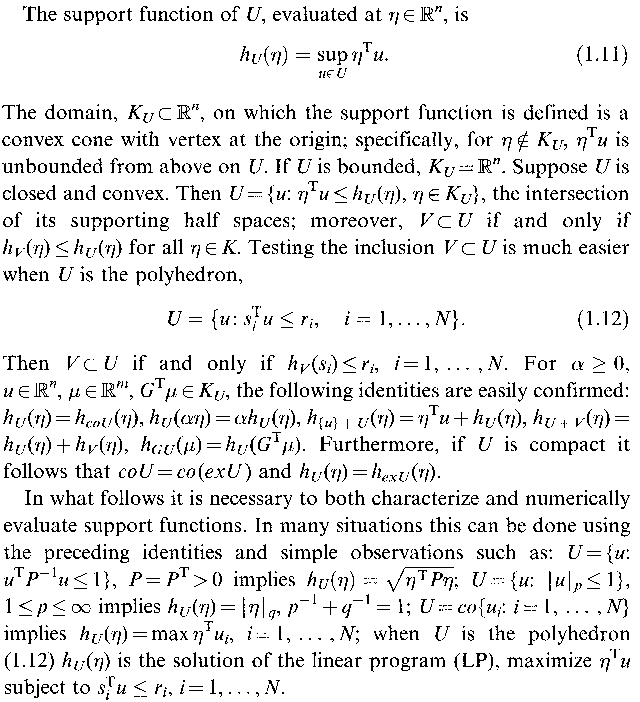
\includegraphics{figs/support1}

\noindent 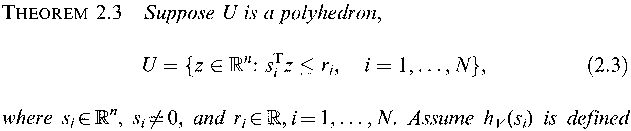
\includegraphics{figs/support31}\\
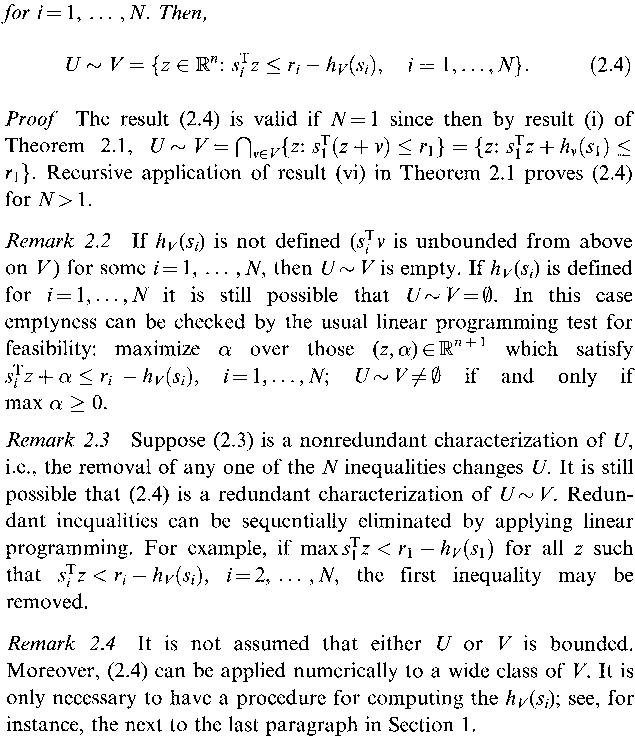
\includegraphics{figs/support32}

\bibliographystyle{IEEEtran}
\bibliography{IEEEabrv,../anytime_ref}

\end{document}
